\section{GIỚI THIỆU VÀ PHÂN TÍCH BÀI TOÁN}
\subsection{Đặt vấn đề và mục tiêu nghiên cứu}
Sơ tán trong công trình nhiều tầng là bài toán phân bổ dòng người trên mạng có tài nguyên hữu hạn. Chiều dài tuyến, khả năng thông hành của cửa và cầu thang, sức chứa khu vực chờ và thời điểm xuất hiện nguy cơ cùng chi phối tính khả thi của lịch di chuyển. Khi nhiều nguồn dân số sử dụng chung một tài nguyên, tối ưu đường đi riêng lẻ chưa bảo đảm tối ưu thời gian hoàn tất hoặc số người thoát của toàn hệ thống.

Nghiên cứu xét tòa nhà A4 của Đại học Phenikaa như một trường hợp ứng dụng. Mặt bằng được biểu diễn bởi đồ thị có hướng, trong đó các khu phòng là nguồn dân số; hành lang, sảnh và cầu thang tạo mạng trung chuyển; các vị trí tiếp cận không gian ngoài tại tầng 1 là đích hấp thụ. Biến quyết định gồm phân bổ người theo tuyến và thời điểm thực hiện từng hành động đi hoặc chờ.

Mục tiêu phương pháp luận là tích hợp các thuật toán đồ thị vào một quy trình lập lịch có thể kiểm chứng. Dijkstra xác định tuyến theo thời lượng; luồng cực đại xác định số người thoát tối đa; luồng chi phí nhỏ nhất phân biệt các lịch có cùng lượng thoát và thời hạn. Mô hình mở rộng theo thời gian tạo liên kết giữa quyết định tuyến và ràng buộc năng lực tại từng mốc.

\begin{table}[htbp]\centering\caption{Nội dung nghiên cứu và phương pháp đánh giá}
\small\begin{tabularx}{\linewidth}{P{5.3cm}X}\toprule
Nội dung nghiên cứu & Phương pháp đánh giá\\\midrule
Ảnh hưởng của ràng buộc năng lực & So sánh tuyến cố định M1 với lịch toàn cục M4.\\
Ảnh hưởng của nguy cơ theo thời gian & Thí nghiệm khói tại phòng và cầu thang.\\
Tính nhất quán của lịch & Kiểm tra độc lập và bảo toàn dân số khi phát lại.\\
Phạm vi của kết luận tối ưu & Phân tích giả định, độ nhạy và giới hạn mô hình.\\\bottomrule
\end{tabularx}\end{table}
Đóng góp chính là tích hợp ràng buộc không gian--thời gian và kiểm chứng lịch độc lập với mạng dư của bộ giải.

\topic{Dữ liệu mặt bằng tòa nhà A4}
Bộ dữ liệu nghiên sơ tán được số hóa từ sơ đồ mặt bằng bảy tầng của tòa nhà A4 \cite{map}. Dữ liệu gồm 27 khu phòng với tổng sức chứa tối đa 1.360 người; khu phòng 705 có sức chứa 40 người. Các giá trị này xác định kịch bản đầy tải. Số người hiện diện theo thời khóa biểu hoặc theo quan trắc chưa được đưa vào thực nghiệm.

\begin{figure}[htbp]\centering
\begin{subfigure}{\linewidth}\centering
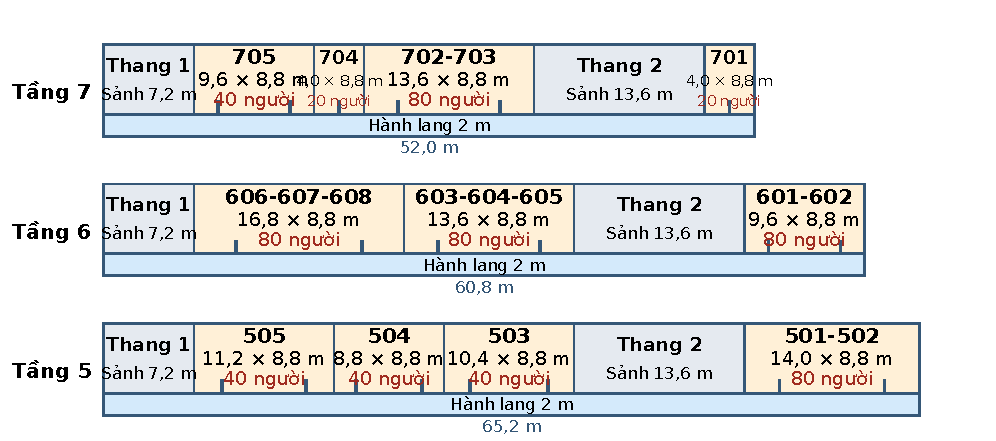
\includegraphics[width=\linewidth]{figures/a4_upper.pdf}
\caption{Các tầng 7--5.}\end{subfigure}
\begin{subfigure}{\linewidth}\centering
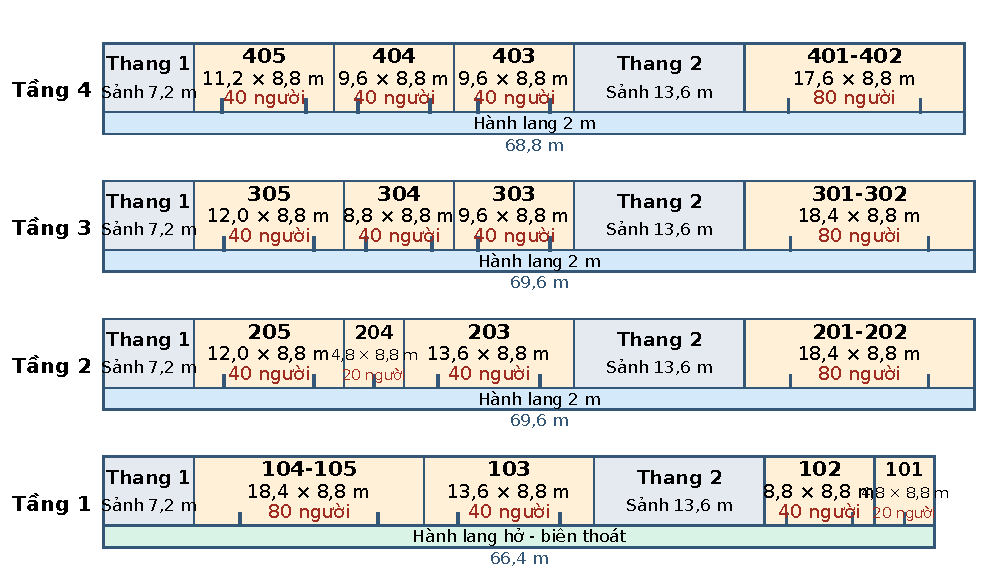
\includegraphics[width=\linewidth]{figures/a4_lower.pdf}
\caption{Các tầng 4--1.}\end{subfigure}
\caption{Mặt bằng tính toán của tòa nhà A4; dữ liệu chi tiết các khu phòng được trình bày tại phụ lục A.}
\label{fig:a4}\end{figure}
Tọa độ cục bộ từng tầng bảo toàn thứ tự và kích thước các khối. Các nút thang cùng chỉ số ở hai tầng kế tiếp được nối bằng quãng đường giữa tầng giả định.

\topic{Phạm vi mô hình và phân loại dữ liệu}
Đơn vị nguồn dân số là khu phòng có nhãn độc lập trong dữ liệu. Các nhãn ghép như 104-105 hoặc 603-604-605 được biểu diễn bởi một nguồn duy nhất với sức chứa của toàn khu. Quy tắc này bảo toàn tổng dân số khi chuyển mặt bằng thành đồ thị, đồng thời tránh đếm lặp các phần của một không gian đã gộp.

\bang{floors}{Đặc trưng hình học và sức chứa theo tầng}

Miền tính toán gồm phòng, cửa phòng, hành lang, sảnh và hai cụm cầu thang. Khu vệ sinh gần cụm thang 2 bị loại khỏi miền: không gán dân số, không tạo đường đi xuyên và không bổ sung diện tích chứa cho sảnh. Các sảnh tiếp cận thang được giữ như những vị trí trung chuyển riêng. Mạng di chuyển chỉ xét phương án sử dụng cầu thang bộ.

Dữ liệu đầu vào được phân thành ba thành phần: đặc trưng mặt bằng và sức chứa; điều kiện biên thoát tại hành lang hở tầng 1; và các tham số động lực học giả định. Thành phần thứ ba gồm bề rộng thông thủy cửa, bề rộng sử dụng vế thang, tốc độ di chuyển, suất thông hành và sức chứa tại các nút. Phân loại này phân biệt đặc trưng hình học với tham số cần hiệu chỉnh thực nghiệm.

Kích thước lõi thang 5 m trong sơ đồ được sử dụng để mô tả hình học. Khả năng thông hành trên thang được tính với bề rộng sử dụng giả định 1,5 m. Hai đại lượng có ngữ nghĩa khác nhau và được lưu riêng để bảo đảm khả năng kiểm soát cấu hình.

\topic{Yêu cầu hệ thống và tiêu chí đánh giá}
Mã nguồn và cấu hình thực nghiệm được công bố tại kho GitHub của nghiên cứu \cite{code}. Hệ thống được triển khai dưới dạng giao diện dòng lệnh, có chức năng sinh dữ liệu, giải lịch, kiểm tra độc lập và xuất kết quả. Mỗi lượt thực nghiệm lưu ảnh chụp mô hình, phân bố dân số, kịch bản nguy cơ, seed, phiên bản phần mềm và lịch hành động. Trực quan hóa được suy xuất từ lịch đã kiểm chứng để duy trì tính nhất quán với nghiệm tối ưu.

\begin{table}[htbp]\centering\caption{Các điều kiện kiểm chứng của hệ thống}
\small\begin{tabularx}{\linewidth}{P{1cm}P{4cm}X}\toprule
Mã & Điều kiện & Tiêu chí kiểm chứng\\\midrule
R1 & Nhất quán dữ liệu mặt bằng & 7 tầng, 27 khu phòng, 1.360 người; khu 705 có 40 người.\\
R2 & Đúng điều kiện biên & 7 cửa phòng tầng 1 và 2 vùng thoát từ sảnh thang.\\
R3 & Khả thi về năng lực & Lưu lượng cạnh và lượng chứa nút không vượt giới hạn.\\
R4 & Khả thi về thời gian & Mọi hành động kết thúc trước thời điểm mất an toàn.\\
R5 & Bảo toàn dân số & Tổng ở nút, đang đi, đã thoát và phơi nhiễm bằng đầu vào.\\
R6 & Khả năng tái lập & Lưu đủ cấu hình, lịch và kết quả kiểm tra.\\\bottomrule
\end{tabularx}\end{table}

Tiêu chí được áp dụng theo thứ tự ưu tiên: lượng người thoát; thời điểm thoát cuối của lượng này; và tổng thời điểm thoát. Thời gian trung bình được báo cáo đồng thời với số người thoát để tránh sai lệch diễn giải khi các phương pháp có tỷ lệ hoàn tất khác nhau.

Các giới hạn về dữ liệu, hành vi và thông tin nguy cơ được tổng hợp tại mục 5.8.

\topic{Tổng quan nghiên cứu và vị trí của mô hình}
Ford và Fulkerson \cite{ford} xét bài toán cực đại hóa lượng vận chuyển trong một khoảng thời gian khi mỗi cạnh có thời lượng và năng lực. Điểm cốt lõi là năng lực được khai thác lặp theo thời gian, vì vậy luồng tĩnh riêng lẻ chưa mô tả được lịch khởi hành. Mạng TEN sử dụng trong nghiên cứu kế thừa cách gắn thời gian vào trạng thái, đồng thời bổ sung sức chứa nút và mốc mất an toàn.

Chalmet, Francis và Saunders \cite{chalmet} xây dựng các mô hình mạng cho sơ tán công trình, liên kết cách biểu diễn không gian với số người thoát và thời điểm thoát. Tổng quan của Dhamala \cite{survey} phân biệt các lớp luồng cực đại, luồng chi phí nhỏ nhất, luồng nhanh nhất và luồng đến sớm. M4 sử dụng thứ tự ưu tiên về lượng thoát, thời điểm thoát cuối và tổng thời điểm thoát; việc tối ưu tổng thời điểm không đồng nghĩa tối ưu mọi tiền tố của đường cong tích lũy.

Các cấu trúc mạng dư, luồng cực đại và chi phí giảm được hệ thống hóa trong Ahuja, Magnanti và Orlin \cite{ahuja}. Trong bài toán A4, mạng dư phục vụ hiệu chỉnh phân bổ giữa nhiều nguồn phòng; potentials cho phép dùng đường ngắn nhất khi cạnh ngược xuất hiện chi phí âm. Sự kết hợp này tạo một mô hình điều phối thay vì ghép độc lập các tuyến ngắn nhất.

Khác biệt của trường hợp nghiên cứu là bảy cửa phòng tầng 1 kết thúc trực tiếp ở biên ngoài, trong khi dân số tầng trên phải qua hai hệ thang. Do đó, dân số tầng 1 không được cộng vào lưu lượng bắt buộc qua lát cắt cầu thang. Phân biệt này được sử dụng khi xây dựng cận dưới và phân tích nút thắt ở phần thực nghiệm.

\topic{Bố cục báo cáo và kế hoạch phân công}
Phần 1 xác lập bài toán và dữ liệu. Phần 2 trình bày đồ thị, ràng buộc và hàm mục tiêu. Phần 3 mô tả các thuật toán cùng lập luận tính đúng đắn. Phần 4 trình bày cài đặt và kiểm chứng. Phần 5 phân tích kết quả, đối chứng bổ sung, độ nhạy và giới hạn. Các phụ lục lưu danh sách khu phòng, ký hiệu và dấu vết dữ liệu.

\begin{table}[htbp]\centering\caption{Kế hoạch phân công nhiệm vụ trong nhóm}
\small\begin{tabularx}{\linewidth}{P{3cm}X}\toprule
Thành viên & Phạm vi phụ trách\\\midrule
Lý Thành Đạt & Tích hợp mô hình đồ thị, bộ tối ưu M4 và kiểm tra tính nhất quán của kết quả.\\
Đinh Đức Mạnh & Chuẩn hóa dữ liệu mặt bằng, mô hình nguy cơ và các phương pháp đối chứng.\\
Phạm Văn Đạt & Thiết kế thực nghiệm, trực quan hóa, tổng hợp bảng và biên tập nội dung.\\\bottomrule
\end{tabularx}\end{table}
Đây là kế hoạch phân công; việc rà soát số liệu và kết luận được thực hiện chung.
